\documentclass[tikz]{standalone}
\usetikzlibrary{positioning,calc}
\begin{document}
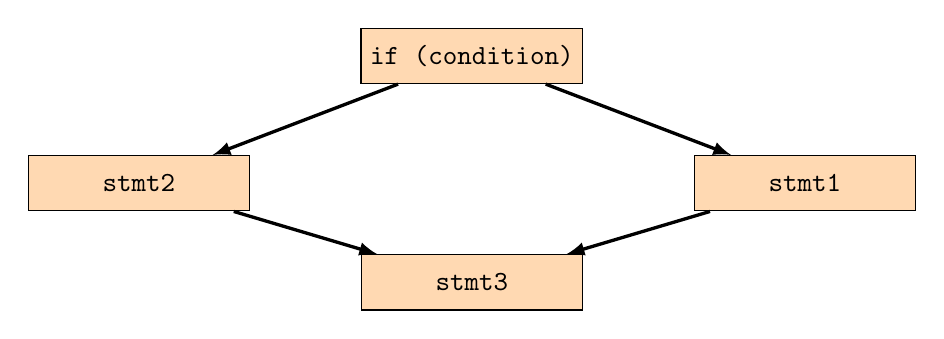
\begin{tikzpicture}[node distance = 9mm and 14mm,
  nodes={draw, fill=orange!30, minimum width=8em, minimum height=2em,
    font=\ttfamily},
  arr/.style = {very thick,-latex}
  ]
  \node (if) {if (condition)};
  \node (true-bb)  [below right=of if] {stmt1};
  \node (false-bb) [below left=of if]  {stmt2};
  \node (end) [below=of $(true-bb)!0.5!(false-bb)$] {stmt3};

  \draw[arr] (if) -- (true-bb);
  \draw[arr] (if) -- (false-bb);
  \draw[arr] (true-bb) -- (end);
  \draw[arr] (false-bb) -- (end);
\end{tikzpicture}
\end{document}
